\documentclass[10pt]{article}
\usepackage{polski}
\usepackage[left=1cm, right=1.5cm, top=0cm, bottom=1cm]{geometry}
\usepackage{multicol}
% \renewcommand{\familydefault}{\sfdefault}
\usepackage{lipsum}
\usepackage{graphicx}
\usepackage[T1]{fontenc}
\usepackage{charter}
\usepackage{enumitem}
\usepackage{fancyvrb}
\usepackage{nopageno}

\begin{document}

    % \hskip-1.55cm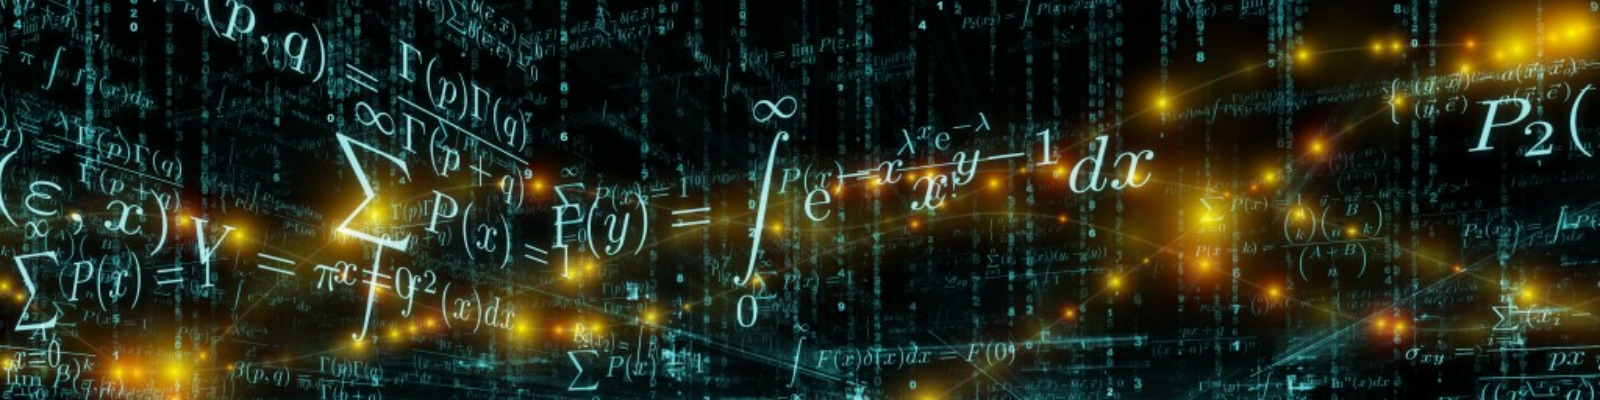
\includegraphics[scale=0.4]{banner.png}
    % \hskip-1.55cm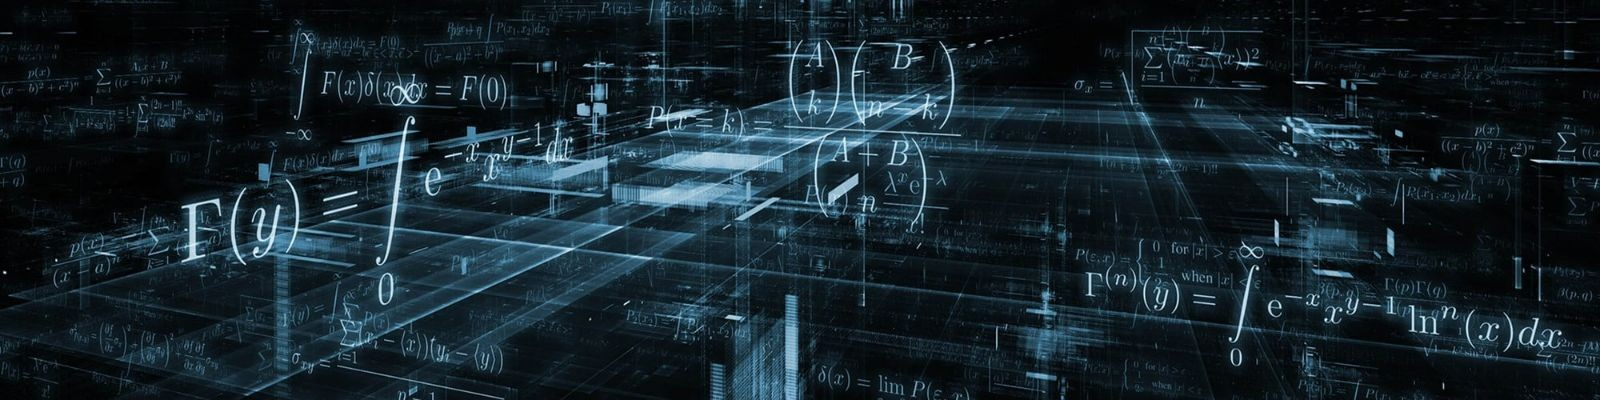
\includegraphics[scale=1.6]{banner4.jpg}
    \hskip-1.55cm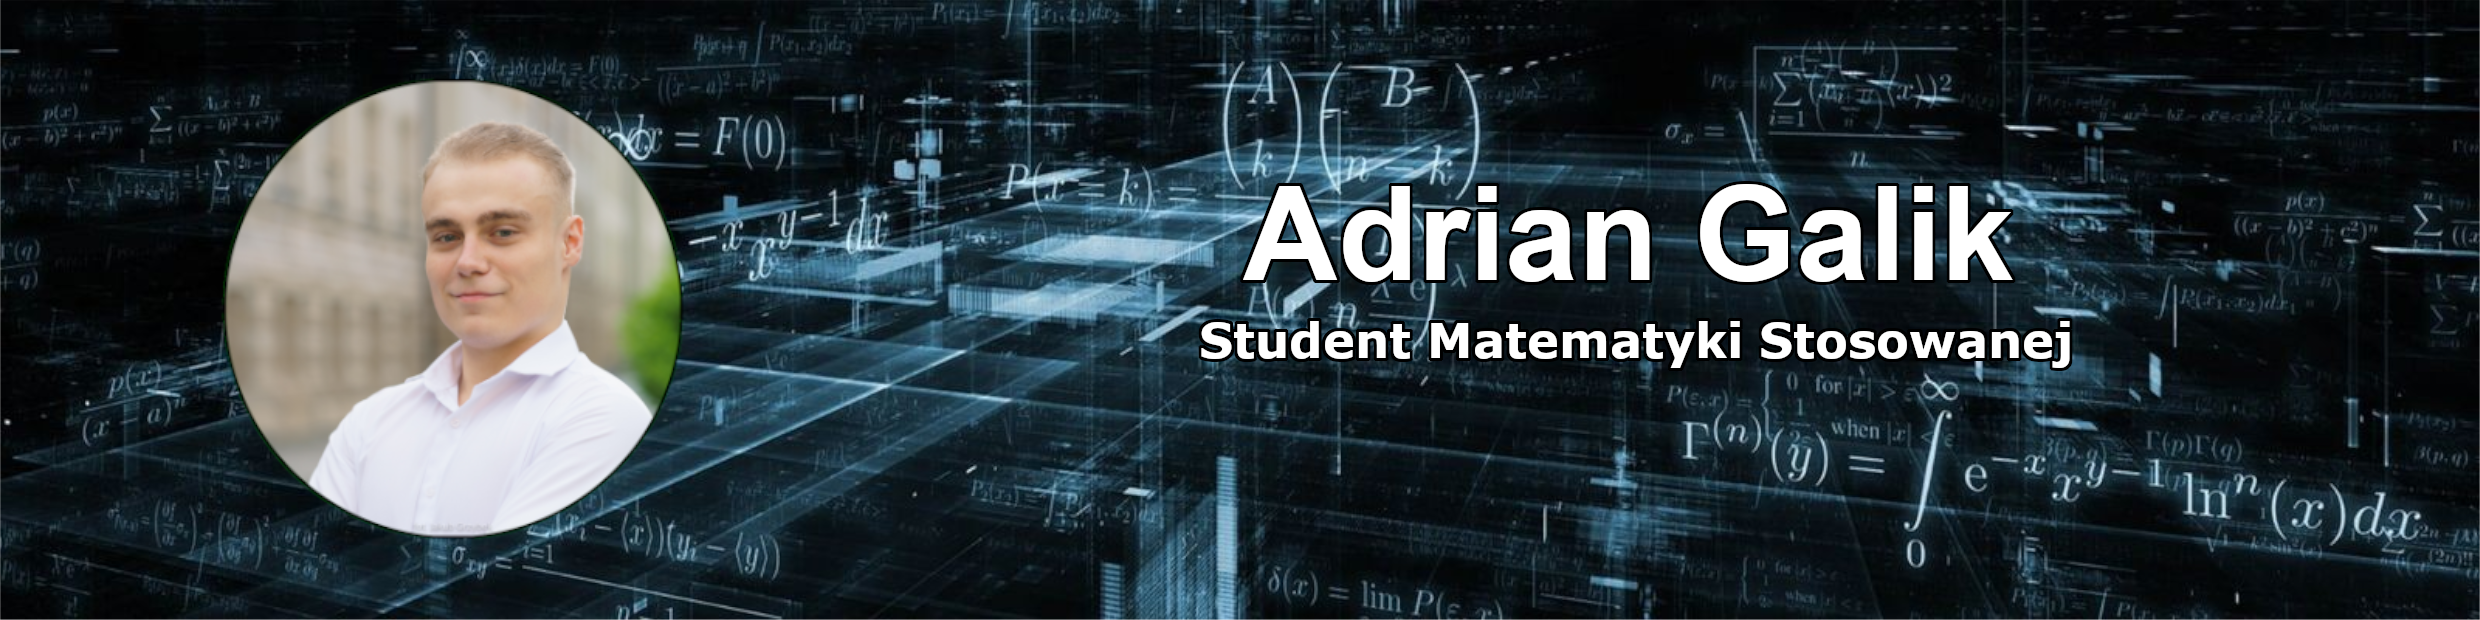
\includegraphics[scale=0.25]{benger.png}
    % \hskip-1.55cm
\includegraphics[scale=1.6]{banner5.jpg}
    % \hskip-1.6cm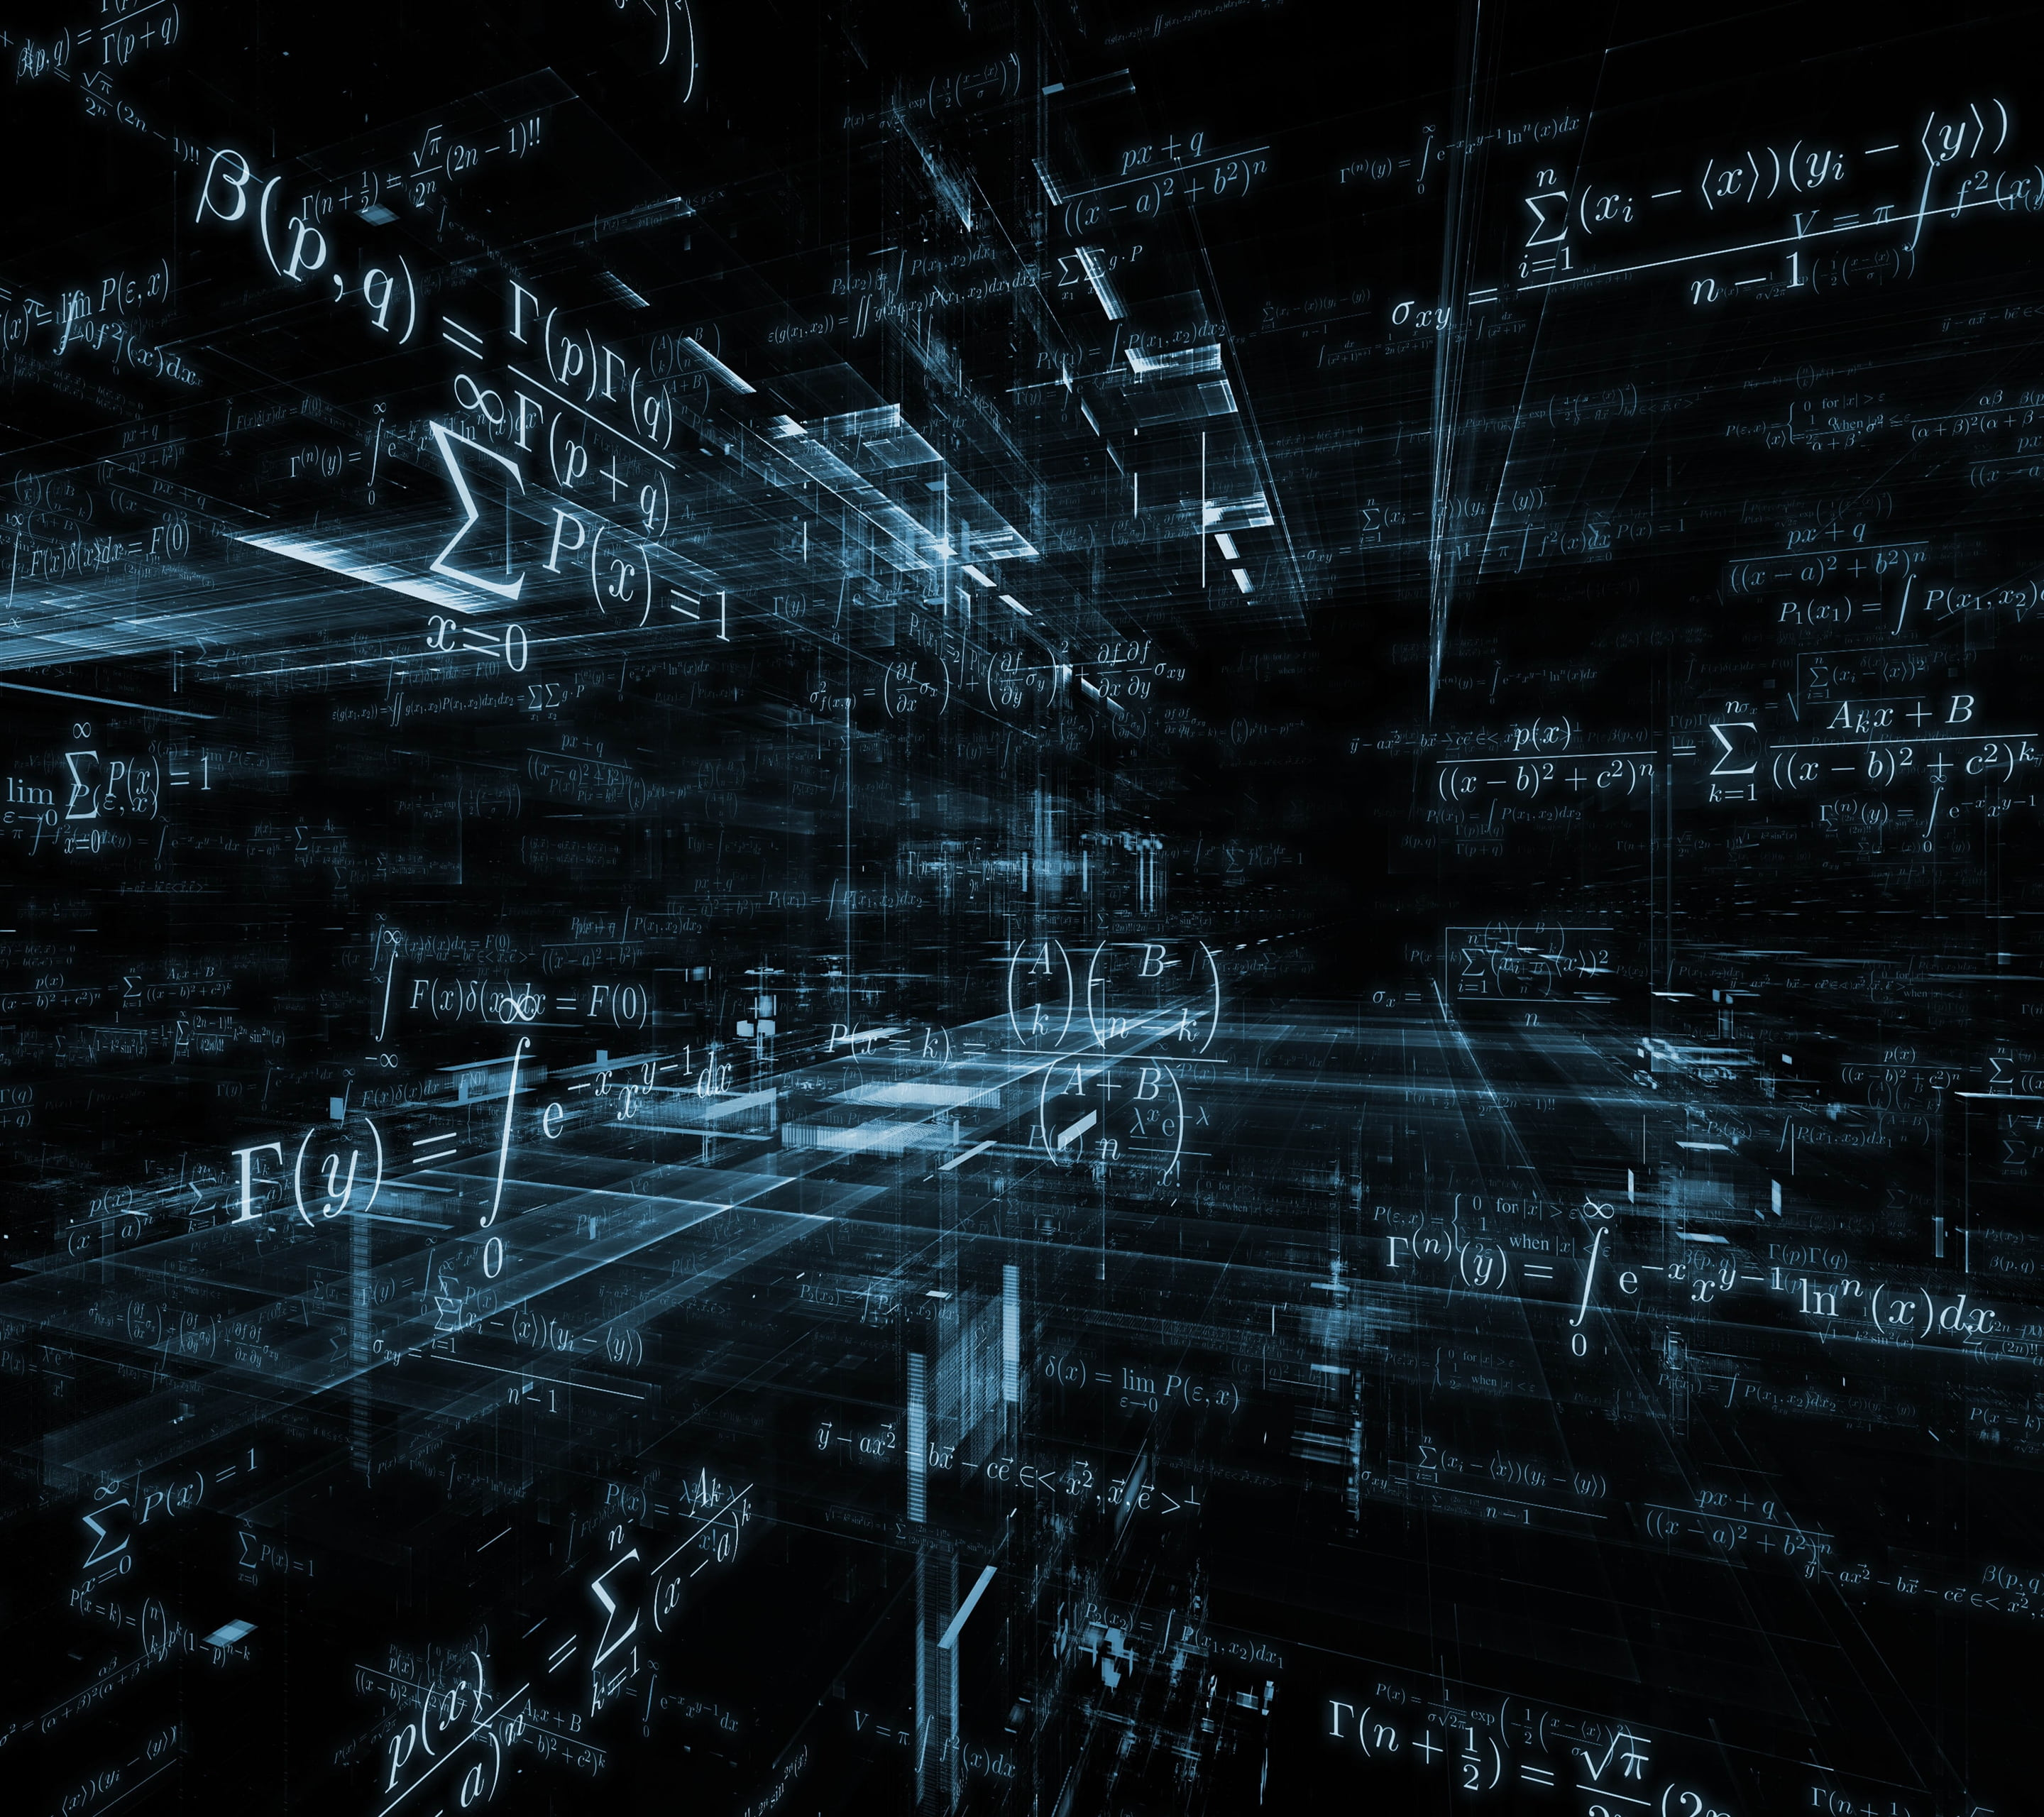
\includegraphics[height=0.20\textheight, width=1.5\textwidth]{banner2.jpg}
    % \hskip-1.6cm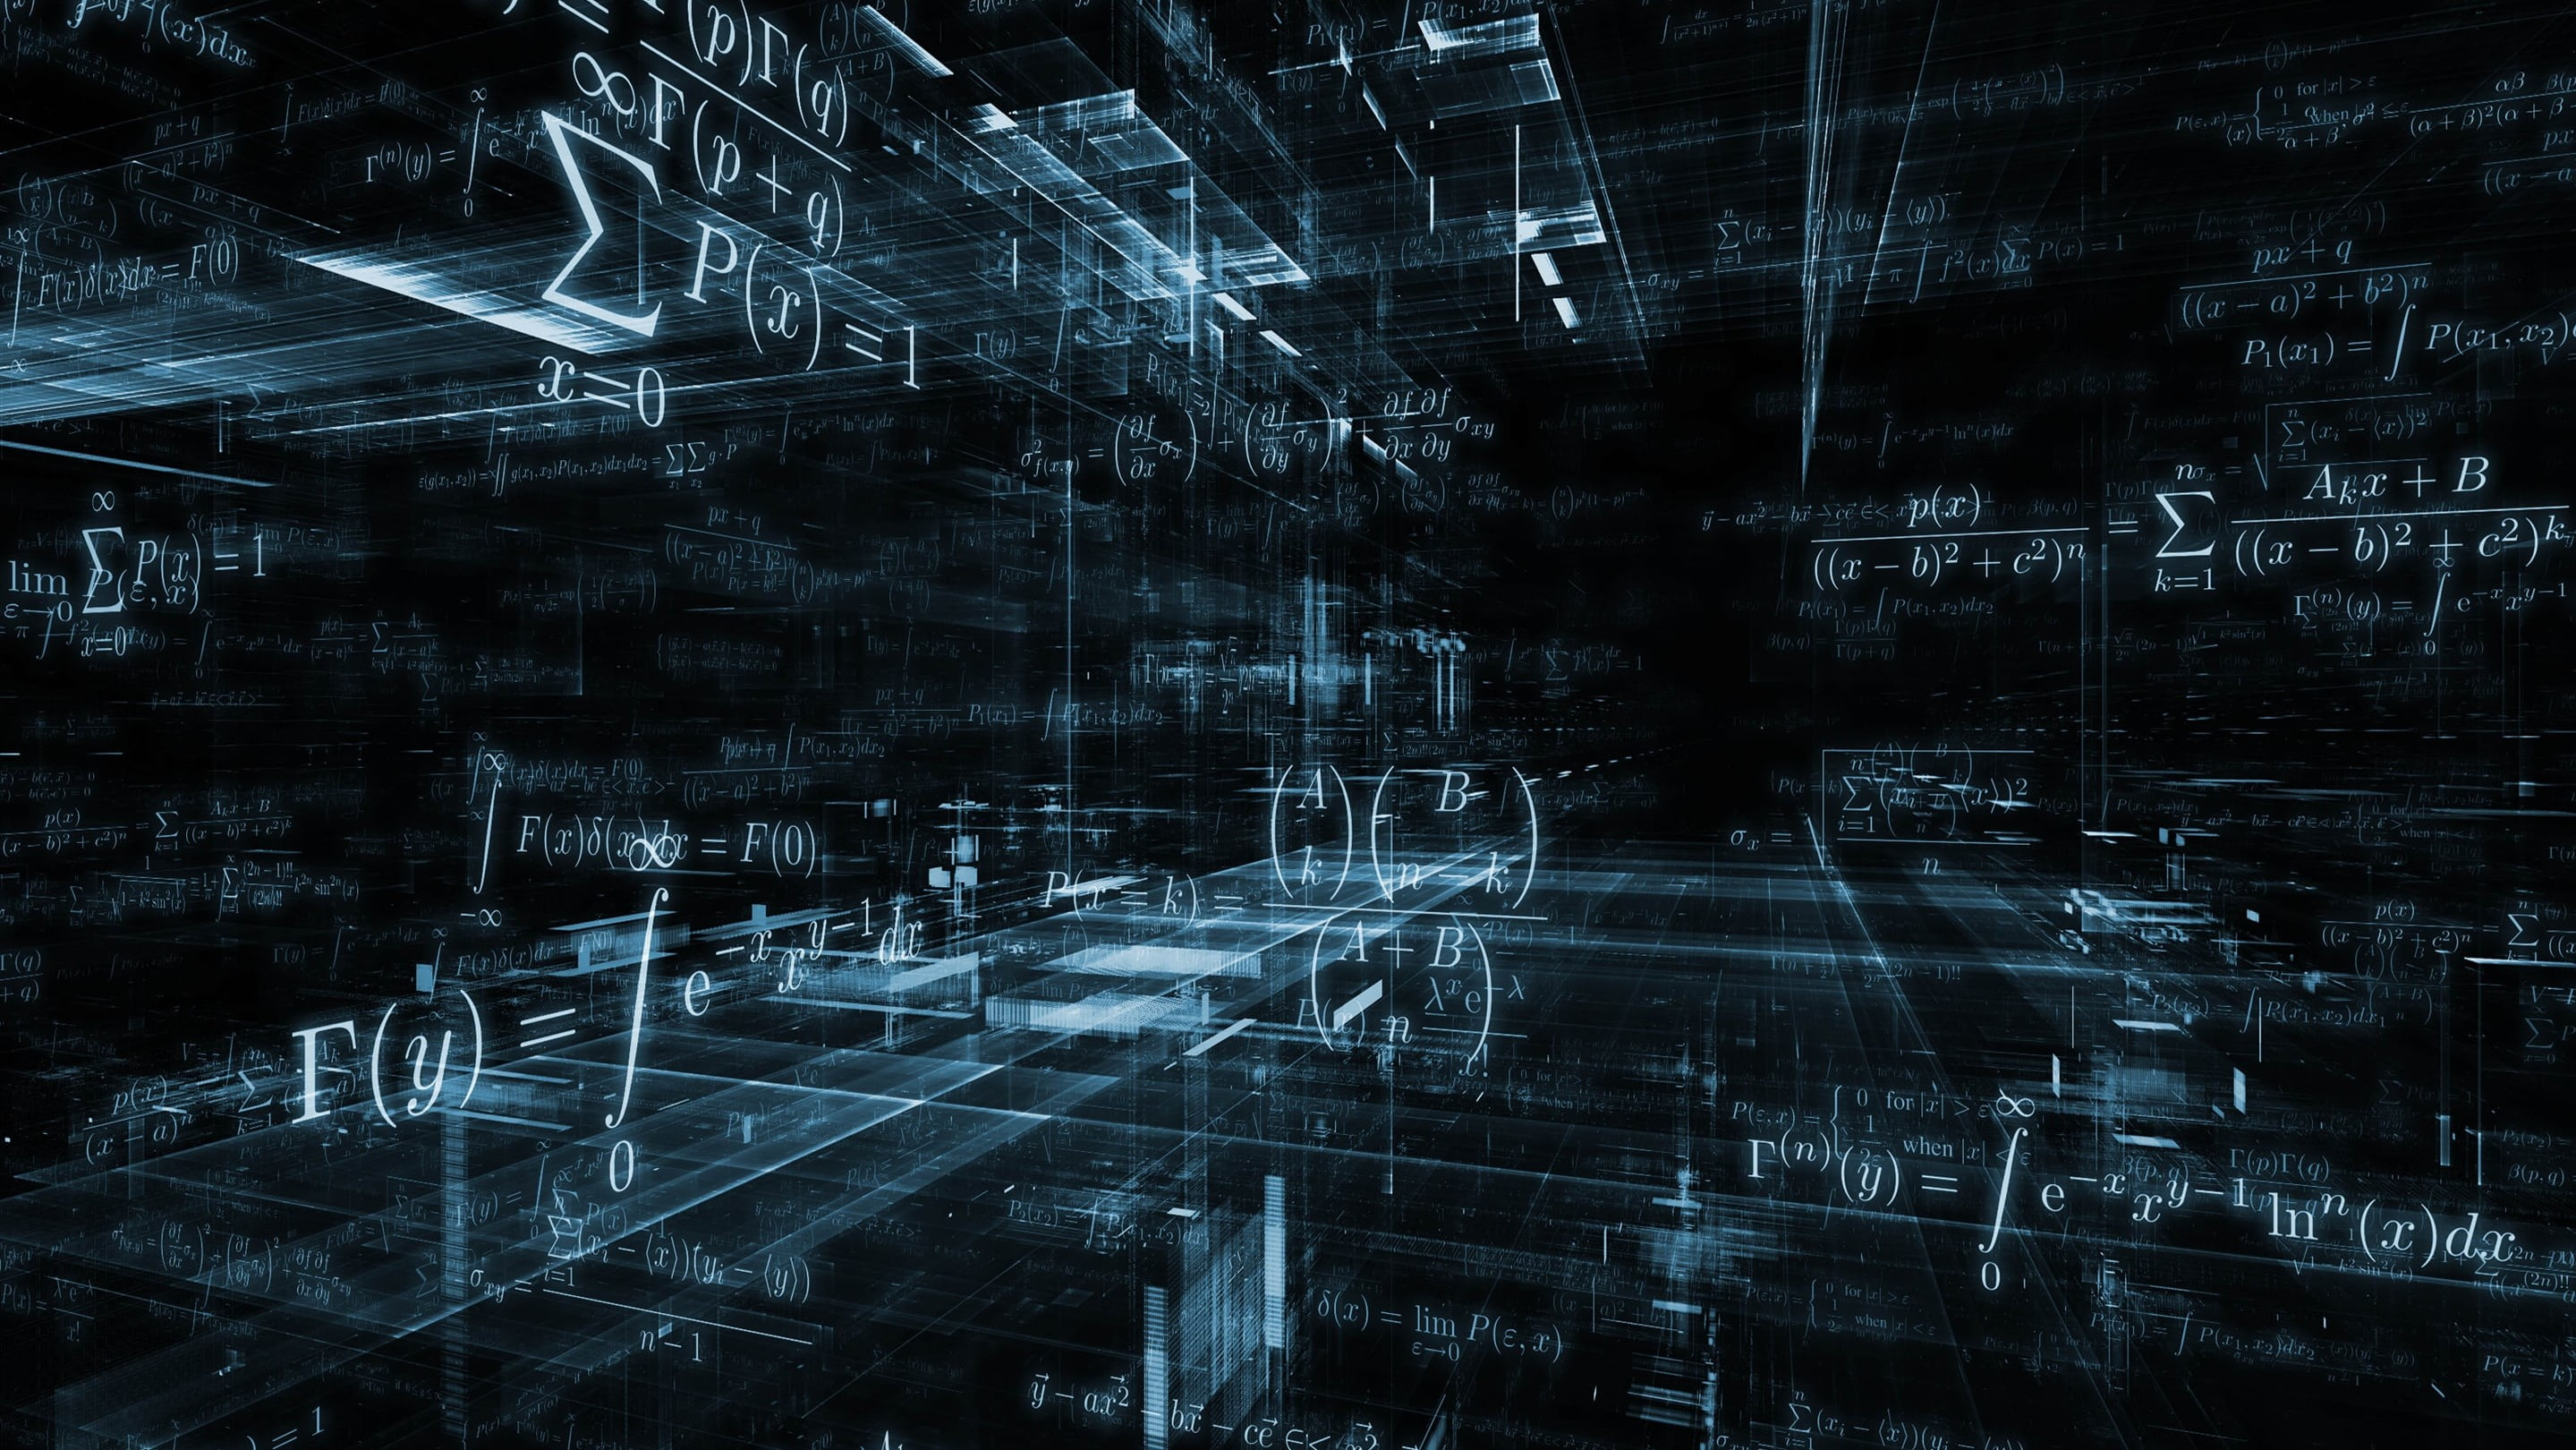
\includegraphics[height=0.25\textheight, width=1.5\textwidth]{banner3.jpg}
    \noindent
    \thispagestyle{empty}

    \vskip+0.4cm\begin{minipage}[t]{0.30\textwidth}
        \textbf{+48 663 383 000 \\
        adriangalik123@gmail.com} \\ \\
        \rule{6cm}{1pt} \\ \\
        \fontsize{14pt}{14pt}{\textbf{SKILLS:}}
        \fontsize{10pt}{10pt}
        \begin{itemize}[leftmargin=*]
            \setlength{\parskip}{0pt}
            % \setlength\itemsep{0pt} 
            \item \textbf{Python} intermediate level
            \item Abstract data structures: \textbf{Stacks, Queues, Trees, Graphs}
            \item algorithmics
            \item mathematical models and \\ statistical methods
            \item applications of differential \\ equations
            \item Numerical calculations: \textbf{Julia}
            \item Projektowanie i zarządzanie \\ sieciami komputerowymi
            \item Zarządzanie bazami danych: \textbf{SQL}
            \item Montaż i eksploatacja systemów komputerowych: \textbf{Windows, \\ Linux}
            \item Tworzenie i administrowanie \\ stronami internetowymi: \textbf{HTML, CSS, JavaScript, Flask, PHP}
            \item Język formatowania tekstu: \textbf{LaTeX}
            \item System kontroli wersji: \textbf{Git}
            \item Analityczne myślenie
            % \item Logika matematyczna
            \item Praca zespołowa 
        \end{itemize}
        \rule{6cm}{1pt} \\ \\
        \fontsize{14pt}{14pt}{\textbf{JĘZYKI:}}
        \fontsize{10pt}{10pt}
        \begin{itemize}[leftmargin=*]
            \setlength{\parskip}{0pt}
            % \setlength\itemsep{0pt} 
            \item Polski ojczysty
            \item Angielski C1
        \end{itemize}
        \rule{6cm}{1pt} \\ \\
        \fontsize{14pt}{14pt}{\textbf{ZAINTERESOWANIA:}}
        \fontsize{10pt}{10pt}
        \begin{itemize}[leftmargin=*]
            \setlength{\parskip}{0pt}
            % \setlength\itemsep{0pt} 
            \item Astrofizyka
            \item Matematyka
            \item Uczenie maszynowe
        \end{itemize}
    \end{minipage}
    \hfill % horizontal space between columns
    \begin{minipage}[t]{0.60\textwidth}
        \fontsize{14pt}{14pt}{\textbf{O MNIE:}}
        \fontsize{10pt}{10pt} \\ \\
        Jestem ambitnym studentem \textbf{Matematyki Stosowanej}. Więdzę  \\ matematyczną wykorzystuje do pisania \textbf{algorytmów} oraz do obliczania zagadnień z astrofizyki.
        Moim ulubionym językiem jest \textbf{Python} i chciałbym go wykorzystywać w swojej pracy. W przyszłości widzę siebie w obszarze \textbf{uczenia maszynowego}. \\ \\
        \rule{11cm}{1pt} \\ \\
        \fontsize{14pt}{14pt}{\textbf{DOŚWIADCZENIE:}}
        \fontsize{10pt}{10pt}
        \begin{itemize}[leftmargin=*]
            \setlength{\parskip}{0pt}
            % \setlength\itemsep{0pt} 
            \item Praktyki zawodowe w firmie \textbf{Sports Media}. Sieci i systemy \\ komputerowe
            \item Praktyka zawodowe w firmie \textbf{Zapaśnik IT}. Zarządzanie systemami  \\komputerowymi
            \item Koło naukowe \textbf{Robocik}. Projektowanie sztucznej inteligencji i tworzenie algorytmów sterowania (\textbf{Python})
            \item Członek komisji do spraw Dydaktyki i Praw Studenta
            \item Projekt symulujący układ słoneczny (odziaływania grawitacyjne) \\ poprzez numeryczne rozwiązywanie problemu n-ciał  (\textbf{Python}). 
            \item Projekt rozwiązujący numerczynie (bez użycia bibliotek) równania różniczkowe Friedmana określające ewolucję wszechświata.
            Celem było uzyskanie informacji o wszechświecie tj. wiek, przeszły i przyszły jego rozwój (\textbf{Python})
        \end{itemize}
        \rule{11cm}{1pt} \\ \\
        \fontsize{14pt}{14pt}{\textbf{WYKSZTAŁCENIE:}}
        \fontsize{10pt}{10pt}
        \begin{itemize}[leftmargin=*]
            \setlength{\parskip}{0pt}
            % \setlength\itemsep{0pt} 
            \item \textbf{Politechnika Wrocławska, Wydział Matematyki, Matematyka Stosowana, październik 2021 - nadal}
            \item \textbf{Zespół Szkół Teleinformatycznych i Elektronicznych we Wrocławiu, Technikum nr 7 (Technik Informatyk), wrzesień 2017 - kwiecień 2021} 
        \end{itemize}
        \rule{11cm}{1pt} \\ \\
        \fontsize{14pt}{14pt}{\textbf{CERTYFIKATY:}}
        \fontsize{10pt}{10pt}
        \begin{itemize}[leftmargin=*]
            \setlength{\parskip}{0pt}
            % \setlength\itemsep{0pt} 
            \item \textbf{Kwalifikacja EE.09 - Programowanie, tworzenie i administrowanie stronami
            internetowymi i bazami danych}
            \item \textbf{Kwalifikacja EE.08 - Montaż i eksploatacja systemów komputerowych, urządzeń
            peryferyjnych i sieci}
        \end{itemize}
        \rule{0pt}{0pt} \\ \\ \\ 
        \fontsize{7pt}{5pt}\selectfont  
        Wyrażam zgodę na przetwarzanie moich danych osobowych zawartych w dokumentach aplikacyjnych w
        celu przeprowadzenia postępowania rekrutacyjnego.
        Wyrażam zgodę na przetwarzanie moich danych osobowych w celu wykorzystania ich w kolejnych
        prowadzonych naborach przez okres najbliższych 12 miesięcy
    \end{minipage}

\end{document}